\documentclass{article}
\usepackage{graphicx}
\usepackage[margin=1.5cm]{geometry}
\usepackage{amsmath}

\begin{document}
\twocolumn

\title{Tuesday Warm Up, Unit 1: Filter Design}
\author{Prof. Jordan C. Hanson}
\maketitle

\section{Memory Bank}

\begin{enumerate}
\item \textbf{Recursive filter formula}.  Start with convolution, and let $h[i] = a_i$.  The result is
\begin{equation}
y[n] = \sum_{i=0}^N a_i x[n-i]
\end{equation}
Now add \textit{feedback from prior output samples} to compute the \textit{next} output sample, using coefficients labeled $b_i$.  Note that $b_0 = 0$, as this corresponds to $y[n]$.
\begin{equation}
y[n] = \sum_{i=0}^N a_i x[n-i] + \sum_{i=1}^N b_i y[n-i] \label{eq:1}
\end{equation}
\end{enumerate}

\section{LP and HP Recursive Filters}

\begin{enumerate}
\item \textbf{Low-pass recursive filter}.  (a) Suppose our sampling rate $f_{\rm s}$ is 10 kHz, and the low-pass cutoff frequency $f_{\rm C}$ is 3 kHz.  (b) Find $x = \exp(-2\pi (f_{\rm C}/f_{\rm s}))$. (c) Calculate $a_0 = 1-x$, and $b_1 = x$, with all other $a_i$ and $b_i$ set to zero. (d) Simplify Eq. \ref{eq:1} to account for the constraints on $a_i$ and $b_i$.  (e) Implement this filter in an \verb+octave+ script.
\item \textbf{Low-pass recursive filter}.  (a) Repeat the previous exercise, but for a high-pass recursive filter, using $a_0 = (1+x)/2$, $a_1 = -(1+x)/2$, and $b_1 = x$.  Use $f_{\rm C} = 2$ kHz.  Implement this filter in an \verb+octave+ script.
\end{enumerate}

\section{Isolating AM Signals}

\begin{enumerate}
\item Suppose we are designing a DSP system to isolate the audio data in an AM signal. (a) Create an \verb+octave+ script that mixes (multiplies) a $1.4$ MHz carrier with a $2.5$ kHz audio tone and adds some  gaussian white noise. (b) What frequencies should be present in the spectrum, other than noise? (c) Now \textit{unmix} the signals using an LO (local oscillator) with a frequency equal to the carrier, and use the recursive LP and HP filters from the first two exercises to isolate the signal.
\end{enumerate}

\section{Phase Response}

\begin{enumerate}
\item (a) Create a square pulse in \verb+octave+, and run it through the recursive LP filter. (b) Plot the \textit{phase} of the output versus frequency. (c) Do the same for the LP filter. (d) Are the results \textit{linear} or non-linear?
\item (a) Use the \verb+flipud+ or the \verb+fliplr+ functions in \verb+octave+ to reverse the LP and HP outputs.  (b) Finally, run the \textit{flipped} outputs through the LP and HP filters once more. (c)  Plot the phase versus frequency of each output. (d) Are the results linear?
\end{enumerate}

\begin{figure}
\centering
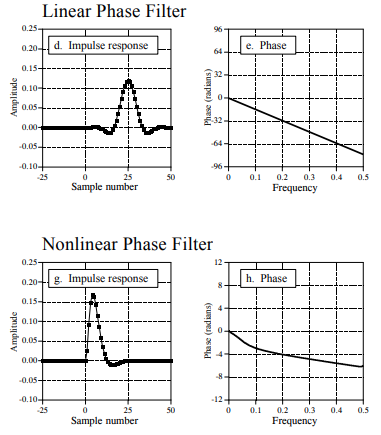
\includegraphics[width=0.5\textwidth]{phase_response.png}
\caption{\label{fig:1} (Top) A linear phase filter has left-right symmetry. (Bottom) A non-linear phase filter does not have left-right symmetry.}
\end{figure}

\end{document}
